%% Capi: En los capítulos 3 y 4 puedes coger texto del documento que tenemos hecho con Giuseppe, y del proyecto tuyo de tesis.
\chapter{Problem Formulation}
\label{ch:ProblemFormulation}
\lettrine[lraise=-0.1, lines=2, loversize=0.2]{A}{s} mentioned in the chapter \ref{ch:Introduction}, the context around which this cognitive task planner is being developed is the inspection and maintenance of electrical networks. Although one of the objectives is to build a task planner whose characteristics allow its easy reuse and adaptation for other applications, it is relevant to state the problem for which it is being originally prepared. 

The AERIAL-CORE project (H2020-ICT-2019-871479) aims to develop different technologies for the use of multi-\gls{UAV} equipment in inspection and maintenance tasks in high-voltage electrical installations. In particular, one of the technologies proposed is the use of aerial co-workers, i.e. small teams of cooperative \glspl{UAV} to safely support maintenance workers while working at height on power lines. These systems would have to interact with humans (see figure \ref{fig:aerial_co_worker}) to inspect certain parts that are indicated to them, monitor worker safety during operation and deliver tools or other light equipment, in order to make the work more efficient and safer. In addition, to have a greater impact, the system would need to operate over extended periods of time, being able to autonomously deal with certain faults or recharges.

\begin{figure}[htbp]
    \centering
    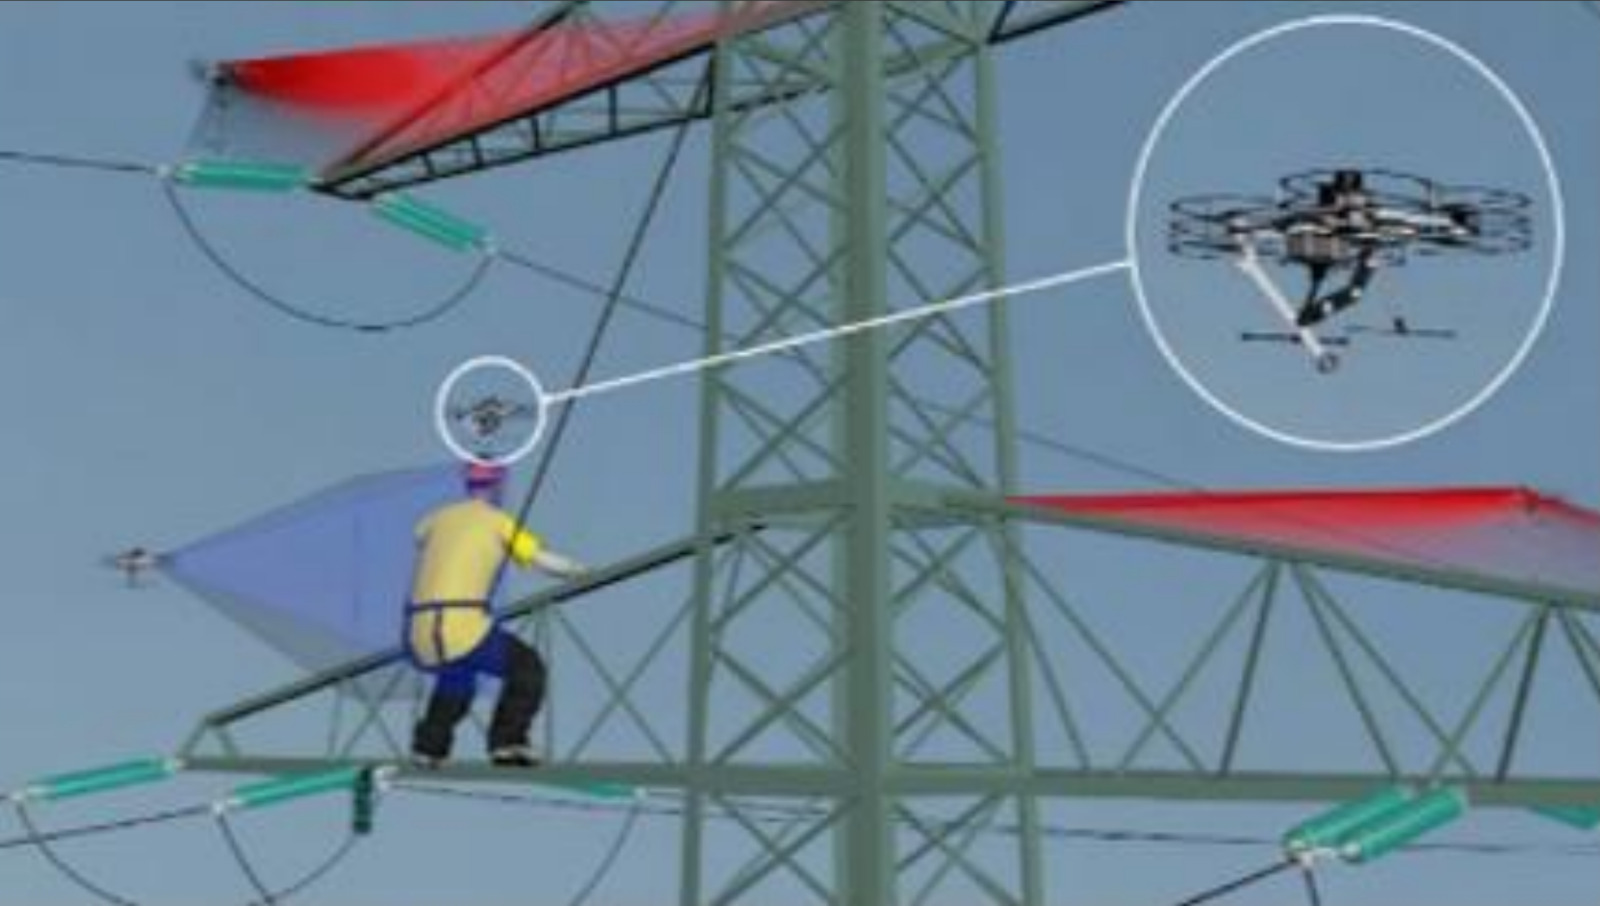
\includegraphics[width=1\linewidth]
    {ProblemFormulation/figures/aerial_co_worker.jpeg}
    \caption{Multi-\gls{UAV} team supporting an operator. Source: \href{https://aerial-core.eu/}{Aerial-Core}}
    \label{fig:aerial_co_worker}
\end{figure}

The mission planning problem with multiple \glspl{UAV} with battery constraints can be posed as an optimization problem, the solution of which indicates the most efficient way to allocate the different tasks and plan recharges. To react to possible failures, one of the most widespread options is to come up with dynamic methods that can replan in real time as certain events occur. Although there are many variants, most formulations for missions where multiple vehicles visit multiple locations to inspect or make deliveries give rise to NP-hard optimization problems and, therefore, the most widespread approach is to solve them using heuristic algorithms.

Uncertainty planning methods are appropriate for adding cognitive capabilities to a system that has to interact with humans in dynamic environments, as they allow optimizing plans by predicting the most likely intentions of humans and the outcomes of future actions. The main problem is their computational complexity, as the plan search space would grow exponentially with the number of \glspl{UAV} and with the future time horizon over which planning is to take place.

It is in this context and with these ideas in mind that the cognitive task planner was developed. As this is one of the software layers that make up the architecture that solve the problem, in order to present the details on which the planner has been designed it is necessary to at least talk about what information exchanges exist between the upper and lower layers of the software architecture, describe the interfaces by which this information travels and highlight when control is passed to lower levels of the software architecture. In the following section this information is presented by individually explaining the different tasks contemplated in the project. 

On the other hand, a review will be made of other important considerations that the planner must take into account such as battery recharges, connection losses and task rescheduling; analyzing the different situations in which each of them can occur and their different causes. 

\section{Description of tasks}
\label{sec:DescriptionOfTasks}

%% A leer y modificar
A leer y modificar (extraido textualmente del WP7 con Giussepe):
This section describes the scenarios proposed for validation of the methodologies and
approaches developed in Work Package (WP) 7. The goal of this WP is to provide the
methods and algorithms that will constitute the core of the software of the Aerial Co-
Workers (ACWs) 1 . The power line inspection problem is taken as motivating example.
Three types of ACWs are referred, each intended to provide different functionality:
Inspection-ACW, Safety-ACW, and Physical-ACW. The use case scenarios can be sum-
marized as follows:
• Inspection, where a fleet of ACWs (i.e., Inspection-ACWs) carries out a detailed
investigation of power equipment autonomously, helping the human workers to
acquire views of the power tower that are not easily accessible (see Fig. 1a);
• Safety, where a formation of ACWs (i.e., Safety-ACWs) provides the supervising
team with a view of the humans working on the power tower in order to monitor
their status and to ensure their safety (see Fig. 1b);
• Physical, where an ACW (i.e., Physical-ACW) physically interacts with the hu-
man worker and provides physical assistance to it, i.e., while in contact with
the human it flies stably, reliably, and accomplishes the required physical task
(e.g., handover of a tool) without becoming harmful for the human worker (see
Fig. 1c).

\subsection{Inspection tasks}
\label{subsec:InspectionTasks}

\subsection{Monitoring tasks}
\label{subsec:MonitoringTasks}

\subsection{Tool delivery tasks}
\label{subsec:ToolDeliveryTasks}


% Otras consideraciones importantes a tener en cuenta: gestíón de la batería, desconexiones, imprevistos, prioridades, tipos de UAV.
% Sacar información del Informe de actividades
\section{Battery recharges}
\label{sec:BatteryRecharges}

\section{Connection losses}
\label{sec:ConnectionLosses}

\section{Task replanning situations}
\label{sec:TaskReplanningSituations}

